\documentclass{article}
\usepackage[utf8]{inputenc}
\usepackage[T1]{fontenc}
\usepackage{graphicx}
\usepackage{hyperref}
\usepackage{geometry}
\geometry{margin=1in}

\title{ESARHADDON}
\date{Encyclopaedia Britannica (1771)}

\begin{document}
\maketitle

\section*{Historical source}
\textbf{Entry ID:} \texttt{entry-esarhaddon-1473} \\
\textbf{Volume ID:} 149979622 \\
\textbf{Character Count:} 490

\subsection*{Extracted Text}
ESARHADDON, the fen of Sennacherib, and his
favorite in the Baylorion of Alfryen. He is faid
have reigned to 9 years at Church, from the year 1904
to 3322; believe which he reigned 13 years at Baby-
ton, in all 8 years. He died in the year of the week
SSS, and was faceded by Sandoshina. Elar-
haddon, in the opinion of Sir Ilane Newton, feems to
be the Shanghai who often, as Catecharina fayo,
old way after the result of Syria, the name \_Bekriamo\_
polar being derived from \_Afrhadon Pal.\_



\section*{Source record}
\begin{itemize}
\item \textbf{Dataset:} \texttt{NationalLibraryOfScotland/encyclopaedia\_britannica\_illustrated}
\item \textbf{Dataset Revision:} \texttt{309f765b1ecc83e0a7f7762e44b4a927a7555443}
\item \textbf{Page ID:} \texttt{britannica:309f765b1ecc83e0a7f7762e44b4a927a7555443:train:1473} \\
  \textbf{Filename:} \texttt{page-1473-b3b602ef6a3d.jpg} \\
  \textbf{Row Index:} 1473 \\
  \textbf{SHA256:} \texttt{b3b602ef6a3d4961...}
\end{itemize}

\begin{figure}[h]
\centering
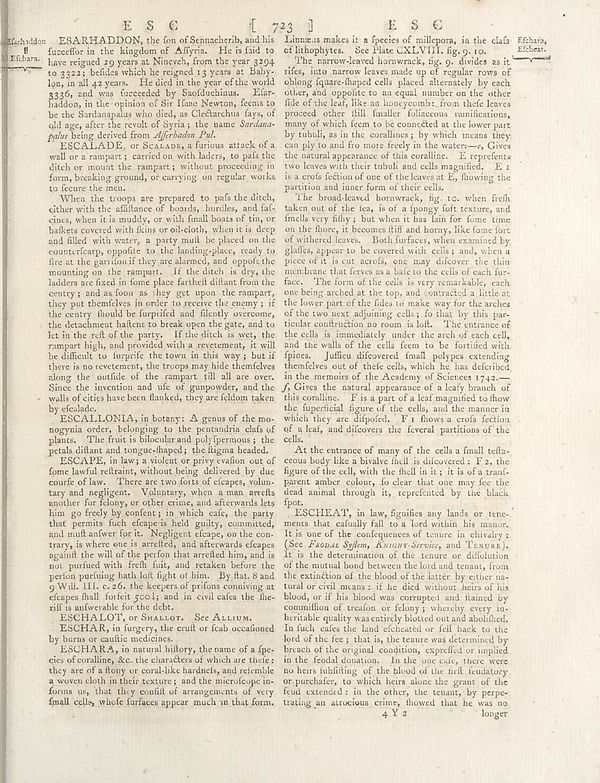
\includegraphics[width=0.85\textwidth]{../scans/page-1473-b3b602ef6a3d.jpg}
\caption*{Source scan: \texttt{page-1473-b3b602ef6a3d.jpg}}
\end{figure}

\end{document}
